\documentclass[12pt, a4paper]{article}
\usepackage[top= 2cm, bottom=2cm, left=2cm, right=2cm]{geometry}
\usepackage[utf8]{inputenc}
\usepackage{url}
\usepackage{hyperref}
\hypersetup{
    colorlinks=true,
    urlcolor=blue,
    linkcolor=blue,
    citecolor=blue
    }
\usepackage{graphicx}
\usepackage[sorting=none]{biblatex} %Imports biblatex package
\addbibresource{bibliography.bib} %Import the bibliography file


\usepackage[breakable]{tcolorbox}
\usepackage{enumerate}
\usepackage[spanish]{babel}
\usepackage{csquotes}
\usepackage{todonotes}

%SIMBOLOS
\usepackage{amsfonts} 
\usepackage{amsmath}
\usepackage{MnSymbol}
\usepackage{wasysym}
\usepackage{marvosym}

\usepackage{amsthm}
\setlength {\marginparwidth }{2cm}

%LISTINGS%%%%%%%%%%%%%%%%%%%%%%%%%%%%%%%%%%
\usepackage{multirow}
\usepackage{xcolor}
\usepackage{listings}
\usepackage{comment}
\usepackage{courier}
%LISTING JAVA%%%%%%%%%%%%%%%%%%%%%%%%%%%%%%%%%%
\definecolor{dkgreen}{rgb}{0,0.6,0}
\definecolor{gray}{rgb}{0.5,0.5,0.5}
\definecolor{mauve}{rgb}{0.58,0,0.82}
\definecolor{gray97}{gray}{.97}

%usando lstdefinestyle {java}{otrasconf} se pueden usar varias diferentes, luego para usarlo \begin{lstlisting}[style=java]
\lstdefinestyle{java}{frame=Ltb,
    language=Java,
    framerule=0pt,
    rulesep=.4pt,
    backgroundcolor=\color{gray97},
    rulesepcolor=\color{black},
    aboveskip=3mm,
    belowskip=3mm,
    showstringspaces=false,
    columns=flexible,
    basicstyle=\small\ttfamily,
    numbers=left,
    numberstyle=\tiny\color{gray},
    keywordstyle=\color{blue},
    commentstyle=\color{dkgreen},
    stringstyle=\ttfamily\color{black},
    breaklines=true,
    breakatwhitespace=true,
    tabsize=3
}
\usepackage{caption}
\DeclareCaptionFormat{listing}{\rule{\dimexpr\textwidth+0pt\relax}{0.4pt}\par\vskip1pt#1#2#3}
\captionsetup[lstlisting]{format=listing,singlelinecheck=false, margin=0pt, font={sf},labelsep=space,labelfont=bf}

\renewcommand\lstlistingname{Código}

\DeclareMathVersion{sans}
\SetSymbolFont{operators}{sans}{OT1}{cmbr}{m}{n}
\SetSymbolFont{letters}  {sans}{OML}{cmbrm}{m}{it}
\SetSymbolFont{symbols}  {sans}{OMS}{cmbrs}{m}{n}
\lstnewenvironment{sflisting}[1][]
  {\lstset{#1}\mathversion{sans}}{}
%%%%%%%%%%%%%%%%%%%%%%%%%%%%%%%%%%%%%%%%%%%%


\begin{document}
\titlepage

\title{\textbf{Diseño de algoritmos}\\
%\vspace{2mm}
\large{\textbf{Trabajo Práctico 1 - Algoritmos sobre Grafos}}
%\vspace{3mm}
\author{
Manuel Latorre FAI-1931\\ manuel.latorre@est.fi.uncoma.edu.ar\vspace{3mm}\\
}}
\date{Segundo cuatrimestre 2022}

\maketitle
\vspace{25mm}
\vfill
\hspace*{-0.1in}{

\includegraphics[width=7cm, scale=0.5]{Images/Unco/faiLogo.png}
\hspace*{1.5in}

\includegraphics[width=5cm, scale=0.5]{Images/Unco/Unco logo.png}
}

\thispagestyle{empty}
\titlepage
\newpage
\tableofcontents %%Indice
\newpage
\pagestyle{plain}
\thispagestyle{plain}
\pagebreak
\section{Punto 1}
\begin{enumerate}[a)]
  \item \textit{Cómo se comportaría el algoritmo de Ordenamiento por Conteo si en el arreglo original se permiten elementos repetidos?}

  En la figura \ref{fig:Traza ordenamiento por conteo} se plantea una traza de ejemplo de como funciona el algoritmo de ordenamiento por conteo con elementos repetidos (en su descripción ademas se encuentra una referencia al repositorio donde se puede ver la imagen mas grande en caso de ser necesario)

  \begin{figure}
    \centering
    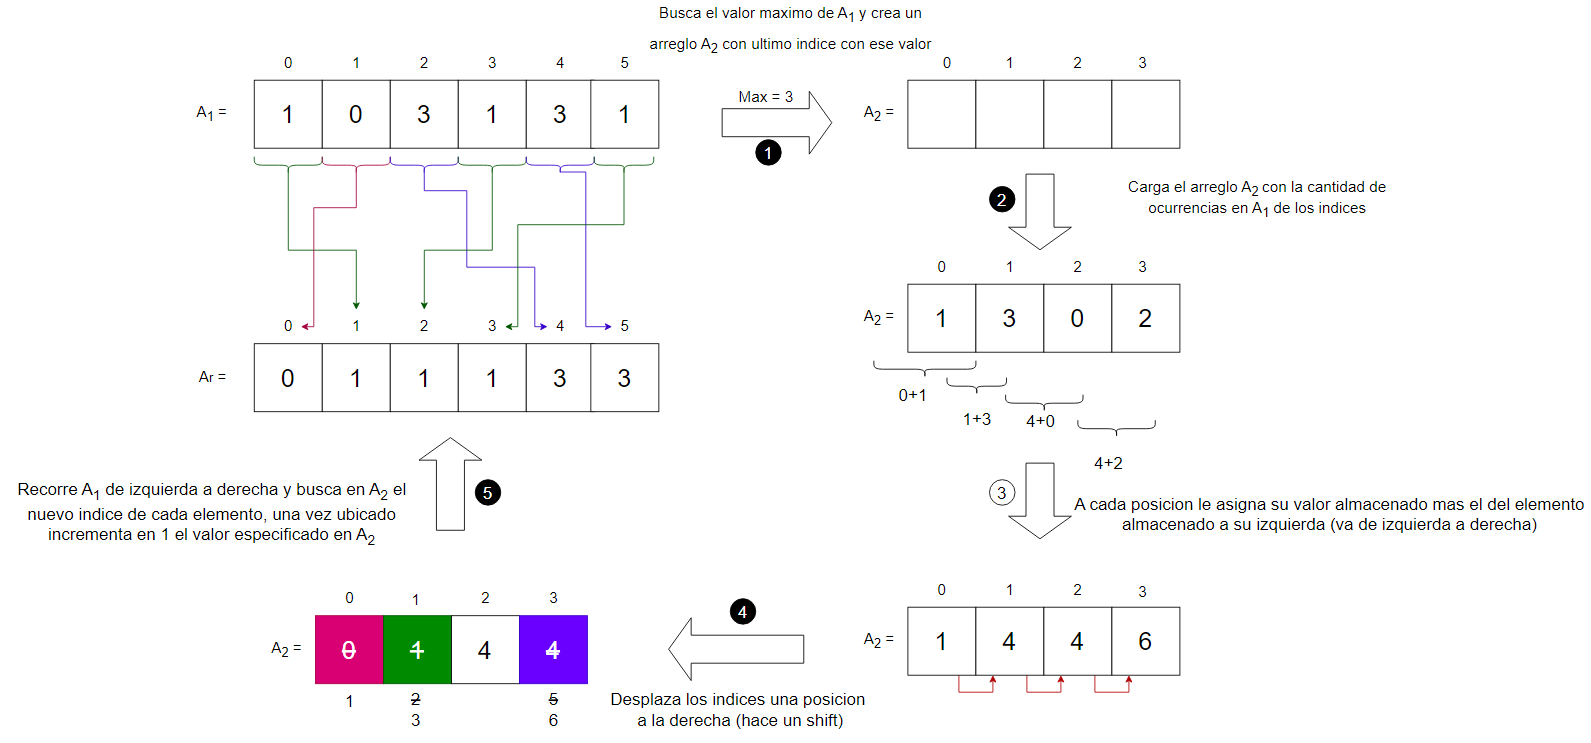
\includegraphics[width=\textwidth, scale=1]{Images/Punto1/Traza ordenamiento por conteo.png}
    \caption{Traza de algoritmo de ordenamiento por conteo \textbf{(imagen en alta resolución en \cite{trazaConteo})}}
    \label{fig:Traza ordenamiento por conteo}
  \end{figure}




  \item \textit{Modificar el algoritmo de Ordenamiento por Conteo para poder ordenar un arreglo de caracteres,
  de tal manera, que sean indistintas las letras mayúsculas y minúsculas, es decir que siempre se cumpla
  que:}\\
  $a<b$,\\
  $a<B$,\\
  $A<b$,\\
  $A<B$,\\
  \textit{En el arreglo resultante debe figurar cada letra en el mismo modo que en el arreglo original.}\\

  Para la implementación los únicos cambios respecto a un algoritmo planteado para números enteros serán la utilización el método \path{Character.compare()} para comparar caracteres y el método \path{Character.toLowerCase()} para convertir caracteres a minúsculas y asi realizar todas las comparaciones logrando la in-distinción entre letras mayúsculas y minúsculas pedida

  \begin{lstlisting}[style=java,caption= Metodo ordenarPorConteoChar]
    public static char [] ordenarPorConteoChar(char [] C){
      int n = C.length;
      int [] count = new int [n];
      char [] sorted = new char[n];
      for (int i = 0; i < n; i++) {
        count[i] = 0;
      }
      for (int i = 0; i < n-1; i++) {
        for (int j = i+1; j < n; j++) {
          if(Character.compare(Character.toLowerCase(C[i]), Character.toLowerCase(C[j]))<0){
            count[j]++;
          }else{
            count[i]++;
          }
        }
      }
      for (int i = 0; i < n; i++) {
        sorted[count[i]]=C[i];
      }
      return sorted;
    }
   \end{lstlisting}

\end{enumerate}
\newpage
\section{Punto 2}

\textit{Para buscar, mediante el algoritmo de Horspool, un patrón de longitud m en un texto de longitud n, con $n \leq m$, dar un ejemplo para: 
\begin{itemize}
  \item Mejor caso.
  \item Peor caso.
\end{itemize}
}

El algoritmo de Horspool es una version simplificada del algoritmo Boyer-Moore utilizando una única tabla. Este pre-procesa el patron que se desea encontrar generando una tabla de desplazamiento que determina cuanto desplazar el patron cuando ocurre un fallo \ref{fig:horspool tabla}.

\begin{figure}
  \centering
  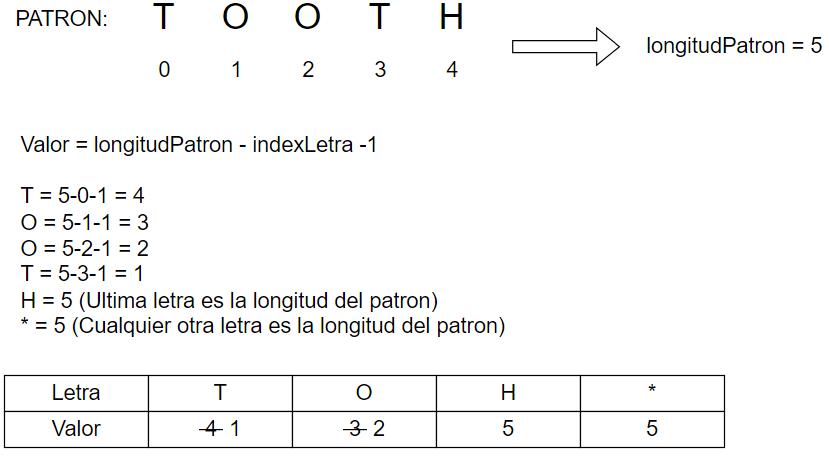
\includegraphics[width=\textwidth, scale=1]{Images/Punto2/Horspool Tabla.png}
  \caption{Ejemplo de creación de tabla de errores}
  \label{fig:horspool tabla}
\end{figure}

Siempre realizaran los desplazamientos basados en el carácter del texto c alineado con el ultimo carácter comparado (fallo) en el patron de acuerdo a la entrada a la tabla de desplazamiento para c \ref{fig:horspool traza}.\\

\begin{figure}[!htb]
  \centering
  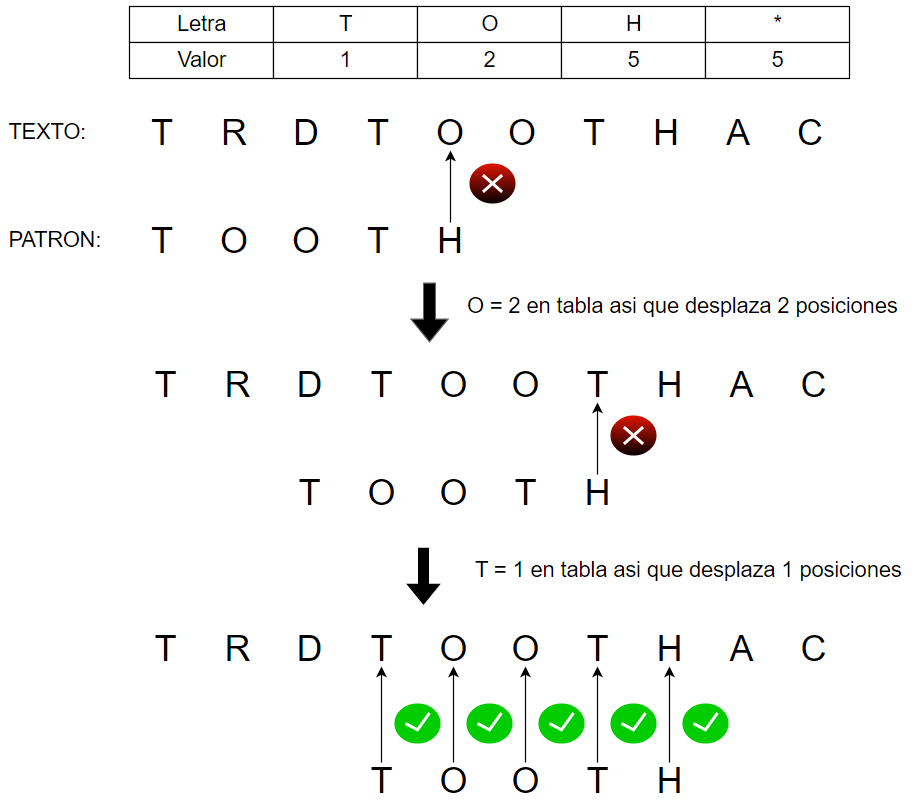
\includegraphics[width=\textwidth, scale=1]{Images/Punto2/Horspool traza.png}
  \caption{Traza de búsqueda de patron con algoritmo de Horspool}
  \label{fig:horspool traza}
\end{figure}


\textbf{Análisis de eficiencia:}
\begin{itemize}
  \item El peor caso sera un patron en el cual coinciden todos los caracteres excepto el primero por ejemplo:
  \begin{itemize}
    \item $1^n$ texto de entrada (longitud n)
    \item $0111\ldots 1$ patron (longitud m)
  \end{itemize}
  En este caso se chequearan constantemente los $m$ caracteres del patron por lo que se tendrá en el peor caso, es decir cuando se hagan desplazamientos de a una posición al encontrar el fallo, un tiempo de ejecución $O(nm)$.

  \item El mejor caso sera cuando el texto de entrada no contenga caracteres del patron por ejemplo:
  \begin{itemize}
    \item $1^n$ texto de entrada (longitud n)
    \item $0^m$ patron (longitud m)
  \end{itemize}
  esto hará que se produzcan saltos del tamaño del patron, es decir de tamaño $m$, produciendo un tiempo de ejecución $O(m/n)$.
\end{itemize}
\newpage
\section{Punto 3}
\textit{Aplicar la técnica de ramificación y poda al problema de la Asignación de Tareas, utilizando la siguiente tabla con los costos correspondientes:
}
\begin{figure}[!htb]
  \centering
  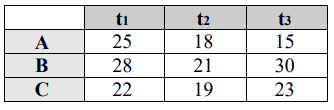
\includegraphics[width=8cm, scale=1]{Images/Punto3/enunciado.png}
  \caption{Tabla de costos}
\end{figure}

Inicialmente se pueden calcular las cotas inferiores y superiores para eliminar posibles casos definiendo un intervalo donde se espera este el resultado, entonces para calcular la cota inferior se tomaran los menores costos de cada fila $A\rightarrow T3 = 15$, $B\rightarrow T2 = 21$, $C\rightarrow T1 = 22$, obteniendo $LB = 15+21+22 = 58$. Luego para la cota superior se puede calcular la sumatoria de la diagonal principal y de la diagonal secundaria y tomar la que de menor resultado, en este caso $DiagonalPrincipal = 25+21+23=69$ y $DiagonalSecundaria = 15+21+22=58$ es decir que $UB = 58$, finalmente se tendrá que el menor resultado estará en el intervalo $[58,58]$ por lo que se deduce que el menor resultado sera 58

Luego se construye un árbol donde a partir de una raíz vacía se van a expandir todas las posibles asignaciones de tareas para A y para cada uno de los nuevos nodos expandidos se calculara su cota inferior nuevamente, luego se expandirá el nodo con menor cota inferior hasta que no queden nodos que puedan expandirse ya que todos los restantes son mayores a la cota inferior del ultimo nodo expandido.

Para el desarrollo de la imagen \ref{fig:poda} a la hora de calcular la cota inferior de cada nodo se obtuvieron los menores costos para cada tarea, es decir se tomo el menor valor de cada columna

\begin{figure}[!htb]
  \centering
  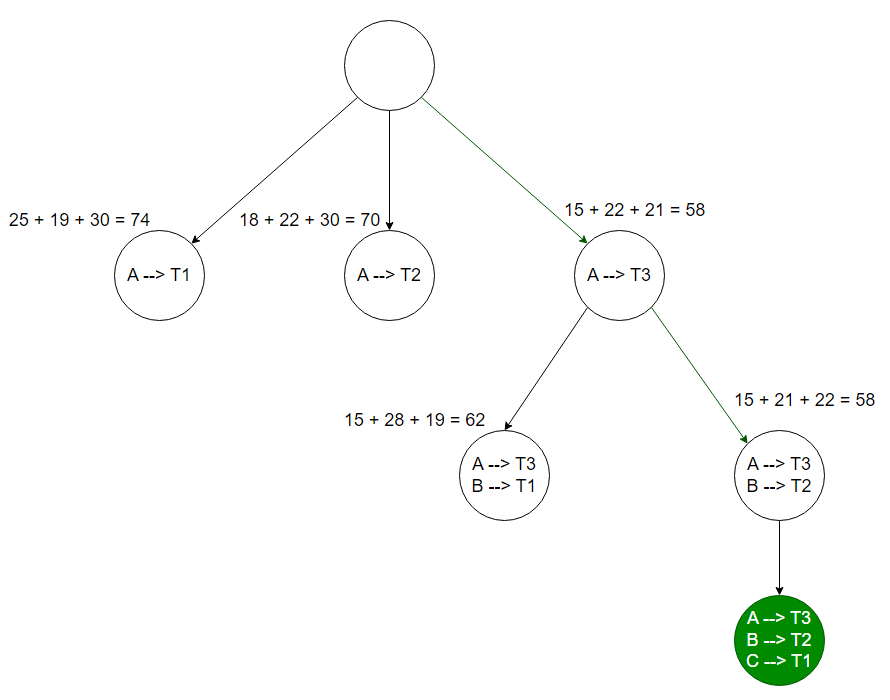
\includegraphics[width=\textwidth, scale=1]{Images/Punto3/Poda.png}
  \caption{Resolución aplicando técnica de ramificación y poda}
  \label{fig:poda}
\end{figure}




\clearpage
\printbibliography
\end{document}